The \emph{flow calculus of mwp-bounds}\index{mwp-calculus}, introduced by~\textcite{jones2009},
is a sound and compositional complexity analysis\index{complexity analysis} technique
for reasoning about variable value growth in imperative programs\index{imperative programs}.
It tracks data-size growth in variables between commands.
The information about variable value growth is captured and expressed as \emph{mwp-bounds}\index{mwp-bound}.

More precisely, for program \pr|C|\symbo{p2} the analysis aims to discover \emph{polynomially bounded data flow relations}\index{data flow relation},
between the \emph{initial values} \(x_1,\ldots,x_n\)\symbo{xpre} of natural-number variables \(\prm{X}_1,\ldots,\prm{X}_n\)\symbo{xvar} and the \emph{final values} \(x'_i\)\symbo{xprime2} of \(\prm{X}_i\) (for \(i=1,\ldots,n\)),
that hold whenever \(\sem{\prm{C}}(x_i \rightsquigarrow x^\prime_i)\)\symbo{flowrel}.
If it is possible to determine that all variable values grow at most polynomially in inputs, the analysis assigns to program \pr|C|\symbo{p2} a \emph{bound}, \ie a conjunction of mwp-bounds\index{mwp-bound};
that characterizes the value growth of all its variables.
The conclusion is derived statically and syntactically by applying inference rules\index{inference rule} to the commands of the program.
As a motivating preview, Examples~\ref{ex:bounds1} and~\ref{ex:bounds2} demonstrate the semantic property the analysis detects.

\begin{example}[Polynomially bounded program]\label{ex:bounds1}
The variable values of the program
\begin{center}
\pr|X1=X2+X3; X1=X1+X1|
\end{center}
are bounded by \(x_1' \leq 2x_2 + 2x_3\)\symbo{xpre}\symbo{xprime2} and \(x_2' \leq x_2\)\symbo{xpre}\symbo{xprime2} and \(x_3' \leq x_3\)\symbo{xpre}\symbo{xprime2}.
Each variable can be bounded by at most a polynomial and the flow calculus\index{mwp-calculus} accepts the program.
The polynomially bounded data flow relation\index{data flow relation} \(\sem{\prm{C}}(x_1,x_2,x_3 \rightsquigarrow x^\prime_1,x^\prime_2,x^\prime_3)\)\symbo{flowrel}
holds for all variables in all program states.
\end{example}

\begin{example}[An always failing program]\label{ex:bounds2}
Consider a program that repeats, for \pr|X2|\symbo{xvar} times, an arithmetic operation on the variable \pr|X1|\symbo{xvar}.
\begin{center}
\pr|X1=1; loop X2 {X1=X1+X1}|
\end{center}
The value of \pr|X2| never changes from its initial value;
therefore, the final value of \pr|X2| is trivially bounded by a polynomial \(x_2' \leq x_2\)\symbo{xpre}\symbo{xprime2}.
However, variable \pr|X1| grows at an exponential rate, with final value bounded by \(x_1' \leq 2^{x_2}\).
Since variable \pr|X1| cannot be bounded by a polynomial, the program is rejected by the flow calculus of mwp-bounds\index{mwp-calculus}.
\end{example}

\subsubsection{Tracking Value Growth With Coefficients}

As a bookkeeping procedure, the flow calculus of mwp-bounds\index{mwp-calculus} tracks
\emph{coefficients}\index{flow coefficient} (or \enquote{flows})
representing how data flows in variables between commands.
The name of the calculus comes from these coefficients.
In the mwp-calculus\index{mwp-calculus}, harmless data flows are acceptable.
However, computations that are harmful lead to values not bounded by a polynomial in the inputs and the coefficients capture these data flow facts.

The coefficients\index{flow coefficient} are, in order of lowest to the highest degree of dependency:
\({0}\)\symbo{zero} indicating no dependency,
\({m}\)\symbo{m} for \emph{m}aximal of linear\index{maximally linear flow},
\({w}\)\symbo{w} for \emph{w}eak polynomial\index{weak polynomial flow},
\({p}\)\symbo{p} for \emph{p}olynomial\index{polynomial flow}, and
\({\infty}\)\symbo{infty} for failure, when no value growth bound can be established.
\noindent The \(m\)\symbo{m}-flow is harmless.
The \(w\)\symbo{w}- and \(p\)-flows are sometimes harmful and have restrictions on their use.
The distinction between \(w\)\symbo{w} and \(p\)\symbo{p} is that \(w\)\symbo{w} is
iteration-independent\index{iteration independence} and \(p\)\symbo{p} is
iteration-dependent\index{iteration dependence} (more harmful).
The \(\infty\)-flow\symbo{infty} is always harmful.
For example, if an exponential dependency exists between two variables,
the analysis assigns an \(\infty\)-coefficient\symbo{infty} to the target variable of the data flow.

Internally, the coefficients\index{flow coefficient} are collected and tracked in \emph{mwp-matrices}\index{mwp-matrix}.
The mwp-matrices are assigned to program commands by the inference rules\index{inference rule} of the \emph{mwp-calculus}\index{mwp-calculus}.
This dissertation will revisit the topic of mwp-matrices\index{mwp-matrix} several times, presenting them at different levels of detail.
For this introduction, it suffices to consider an mwp-matrix\index{mwp-matrix} as an \emph{array of coefficients}\index{flow coefficient} for simplicity.

\paragraph*{A sound calculus of value growth.}
The analysis result is binary and indicates whether all final values can be bounded by polynomials in inputs.
When affirmative, we call the analyzed program \emph{derivable}\index{derivability}.
For a program \pr|C|\symbo{p2} and an mwp-matrix \(M\)\symbo{matrix},
the \emph{syntactic relation}\index{data flow relation} \(\vdash \prm{C} : M\)\symbo{cmat} holds if a program is derivable\index{derivability}.
In other words, a derivable\index{derivability} program can be assigned an mwp-matrix\index{mwp-matrix} of at most $p$\symbo{p}-coefficients at each variable.
If a command \pr|C|\symbo{p2} computes a function growing exponentially, the statement \(\prm{C} : M\) will be false for all matrices \(M\)\symbo{matrix}.
The flow calculus\index{mwp-calculus} result is sound but incomplete.
If a derivable\index{derivability} program terminates\index{termination},
the soundness theorem~\cite[p. 11]{jones2009} guarantees that the variable value growth is polynomially bounded.

\begin{theorem}[{Soundness of mwp-calculus}]\label{mwp-soundness}
\index{soundness theorem of mwp-calculus}
\index{mwp-calculus!soundness theorem}
\(\vdash \prm{C} : \prm{M}\text{ implies } \vDash \prm{C} : \prm{M}\)\symbo{cmat}\symbo{cmatsem}.
\end{theorem}

The soundness theorem connects the syntactic data flow relation\index{data flow relation} to the \emph{semantic property} \(\vDash \prm{C} : M\)\symbo{cmat}.
Informally, derivability\index{derivability} guarantees program \pr|C| has polynomially bounded variable value growth at runtime.
From a complexity-theoretic\index{complexity theory} perspective, this in turn ensures program \pr|C| runs in polynomial time\ccxi{p}~\cite{kristiansen2017}.
The main result of the work introducing the flow calculus\index{mwp-calculus}~\cite{jones2009} is precisely a proof of the soundness theorem.
Since the analysis omits termination\index{termination},
the flow analysis provides a \emph{partial correctness}\index{partial correctness} guarantee.

The flow calculus\index{mwp-calculus} offers no guarantee to programs that are not derivable\index{derivability}.
Then, variable value growth is interpreted as unknown.
A program always fails if a variable value grows \enquote{too fast}, for example exponentially.
A single variable can be the source of whole-program derivation failure.
Alternatively, failure may occur from inability to express satisfiable behavior.
The latter is a built-in limitation of the flow calculus\index{mwp-calculus}.
To increase expressiveness and capture a larger class of derivable\index{derivability} programs,
the mwp-calculus\index{mwp-calculus} includes nondeterminism\index{nondeterminism} in its inference rules\index{inference rule}.
Consequently, a single program may admit multiple derivations with distinct matrices, which in turn complicates determining the result of the analysis.
However, a program is derivable\index{derivability} if there exists a derivation without an \(\infty\)-coefficient.

\paragraph*{The mwp-bounds characterize value growth.}\label{interpreting-bounds}
The column vectors of an mwp-matrix\index{mwp-matrix} encode variable value growth bounds.
An mwp-bound\index{mwp-bound} (denoted \(W,V,U,\ldots\)) characterizes the value growth of a single variable \wrt program inputs.
An mwp-bound\index{mwp-bound} is an expression of form $\max(\vec{x}, \poly_1(\vec{y})) + \poly_2(\vec{z})$.
Variables characterized by $m$-flow are listed in $\vec{x}$; $w$-flows in $\vec{y}$, and $p$-flows in $\vec{z}$.
The notation \(W(\vec{x};\vec{y};\vec{z})\) displays all the variables in an mwp-bound\index{mwp-bound} $W$ where $\vec{x}$, $\vec{y}$ and $\vec{z}$
are respectively the $m$-, $w$- and $p$-variables of \(W\).
Variables characterized by $0$-flow do not occur in the expression and no bound exists if some variable is characterized by $\infty$.
The $\poly_1$ and $\poly_2$ are \textit{honest polynomials}\index{honest polynomial},
build up from constants and variables by applying $+$ and $\times$.
Any of the three variable lists might be empty, and $\poly_1$ and $\poly_2$ may not be present.
When characterizing value growth, an mwp-bound\index{mwp-bound} is approximative;
it excludes precise constants and degrees of polynomials.
We write an mwp-bound\index{mwp-bound} of variable \pr|X| as \(x' \leq W\) where \(x'\) is the final value of \pr|X| and W is an mwp-bound.
A \emph{program bound} is a conjunction (\(\land\)) of its variables' mwp-bounds\index{mwp-bound}.

\begin{example}[Interpreting mwp-bounds]
For an arbitrary variable, the mwp-bound\index{mwp-bound} indicates the final value of the variable is bounded by\ldots

\begin{center}\begin{tabular}{rl}
\(0\) & \ldots a constant. \\
\(\prm{X}\) & \ldots the initial value of variable \pr|X|. \\
\(\max(\prm{X},\prm{Y})\) & \ldots the initial values of \pr|X| or \pr|Y|, the greatest of the two. \\
\(\max(\prm{X},0) + \prm{Y}\) & \ldots the initial values of \pr|X| and \pr|Y|. \\
\(\max(\prm{X0},\prm{X1}+\prm{X2}) + \prm{X3} \times \prm{X4}\) & \ldots the maximum of \pr|X0| or \(\prm{X1}+\prm{X2}\), and \(\prm{X3}\times\prm{X4}\).
\end{tabular}\qedhere\end{center}\end{example}

\noindent Multiple mwp-bounds\index{mwp-bound} of different form can evaluate to the same numerical value.
For example, the mwp-bounds\index{mwp-bound}
\(W \equiv \max(0,\prm{X1}+\prm{X2})+0\) and
\(V \equiv \max(\prm{X1},0)+\prm{X2}\) and
\(U \equiv \max(\prm{X2},0)+\prm{X1}\) are all numerically equal to \(\prm{X1}+\prm{X2}\).
As each variable in the mwp-bound\index{mwp-bound} omits constants.
Thus, an mwp-bound\index{mwp-bound} is best suited for recognizing the \emph{shape} of the value growth rather than its explicit numerical value.
Furthermore, mwp-bounds\index{mwp-bound} can be incomparable.
For example, between \(W \equiv \max(\prm{X1},\prm{X2})+\prm{X3}\) and \(V \equiv \prm{X1}+\prm{X2}\times\prm{X4}\), it is impossible to determine which mwp-bound\index{mwp-bound} evaluates to a lower value numerically.
This means mwp-bounds\index{mwp-bound} cannot be totally ordered.

\subsubsection{Evolution of the Flow Calculus}

A central theme of this dissertation is the gradual technical advancement of the flow calculus of mwp-bounds\index{mwp-calculus}, as those developments are a prerequisite for its different applications.
However, details of these developments are not totally obvious from the publications.
This section presents the technical developments, summarized in~\autoref{tab:evo}.
They correspond to the four publications discussed here in chronological order.

\paragraph*{The original flow calculus.}
The flow calculus of mwp-bounds\index{mwp-calculus}~\cite{jones2009} was designed to characterize sequential imperative polytime programs\index{imperative programs},
with an underlying ambition to study the boundary of decidability~\cite{kristiansen2017}.
The complexity-theoretic\index{complexity theory} result is obtained by bounding the growth of variable values by polynomials in inputs.
In effect, the flow calculus\index{mwp-calculus} provides a computational method \(\mathcal{M}\) for deciding a runtime property,
\begin{gather*}
\mathcal{M}: programs \rightarrow \{yes, no \} \\
\text{ such that } \{C_i \mid \mathcal{M}(C_i) = \text{yes} \} \subset \{ C_i \mid C_i \text{ runs in polynomial time} \}.
\end{gather*}\ccxi{p}
The formulation naturally provides the theoretical foundations and a concrete technique for program analysis.
The analysis is defined over nondeterministic\index{nondeterminism} inference rules\index{inference rule} and coefficients \{0, m, w, p\}\index{flow coefficient} where multiple matrices can be assigned to one program.
A single program has \(3^k\) derivations where \(k\) is the count of binary arithmetic operations (the binary operations are the sources of nondeterminism\index{nondeterminism}).
The analysis proceeds in a \enquote{single-shot}, exploring one derivation path until the complete program syntax has been successfully analyzed, or the derivation fails.
On derivation failure, the analysis restarts to explore a different deprivation path until all paths have been exhausted.

Among the advantage of the original flow calculus\index{mwp-calculus}
is that if a derivation succeeds, the mwp-bounds\index{mwp-bound} are obtained immediately.
Although on success the method produces mwp-bounds\index{mwp-bound} straightforwardly, it does not support searching for mwp-bounds\index{mwp-bound} of specific form.
The mathematical framework is sophisticated and recognizes a larger class of programs than earlier similar systems, \eg~\cite{niggl2006}.
However, beyond pen and paper examples, the technique is infeasible for practical implementation, due to the exponential blowup and inefficient handling of derivation failure.

\paragraph*{The enhanced \textsc{mwp}\(^\infty\)-calculus.}
In an effort to move the flow calculus\index{mwp-calculus} toward practical static analysis,
in~\cite{aubert20222} (\aref{sec:fscd}) the calculus\index{mwp-calculus} was refined to resolve its theoretical inefficiencies.
There are several well-founded motivations for this goal:
a practical analysis permits stress-testing the technique beyond paper examples, exports ideas from implicit complexity to broader communities, and exposes hidden challenges within the analysis technique.

Most notably, the enhanced flow calculus \index{mwp-calculus}\enquote{internalizes}
the nondeterminism\index{nondeterminism} through deterministic inference rules\index{inference rule}.
A key notion is the introduction of the \(\infty\)-coefficient that tracks derivation failure.
Instead of multiple matrices, every program is assigned exactly one (complex) mwp-matrix\index{mwp-matrix}.
The complex mwp-matrix\index{mwp-matrix} captures all derivations at once, in a single data structure, resolving much of the combinatorial inefficiency of the original flow calculus\index{mwp-calculus}.
Program analysis now transforms, from performing multiple derivations, to a question of determining if there exists a derivation without an \(\infty\)-coefficient.
This splits the program analysis procedure into two phases of mwp-matrix\index{mwp-matrix} construction and mwp-matrix\index{mwp-matrix} evaluation.
As a consequence, the mwp-bounds\index{mwp-bound} are no longer immediately obtained from the mwp-matrix\index{mwp-matrix}.

The enhanced flow calculus\index{mwp-calculus} is practically efficient as demonstrated by the prototype implementation, \emph{pymwp}\index{pymwp}\footnote{
    Pronounced \enquote{pa\textsc{i} em double-you p\={e}.}}, visualized in~\autoref{fig:pymwp}.
The technique permits efficient construction of complex mwp-matrices, but only a brute force approach for mwp-matrix\index{mwp-matrix} evaluation.
At the time, the analyzer could answer a question of whether all variables could be bounded (yes/no).
However, in absence of an efficient evaluation strategy, it could not provide concrete bounds (\cf Table 1 in~\aref{sec:fscd}).

\paragraph*{The pymwp static analyzer.}
After continued development, the pymwp\index{pymwp} static analyzer was enhanced in two ways~\cite{aubert2023b}.
The first introduced an efficient mwp-matrix\index{mwp-matrix} evaluation strategy.
It enabled representing all permissible derivations in a compact form and producing an arbitrary instance of a program bound, if at least one bound exists.
The second introduced feedback about source of derivation failure.
This is possible because the \(\infty\)-coefficient marks the locations of failure, yielding a more informative system than the original flow calculus\index{mwp-calculus}.
With these enhancements, the analysis produces results efficiently,
while exceeding the informative capabilities of the original flow calculus\index{mwp-calculus}.

\begin{figure}[t]
\centering
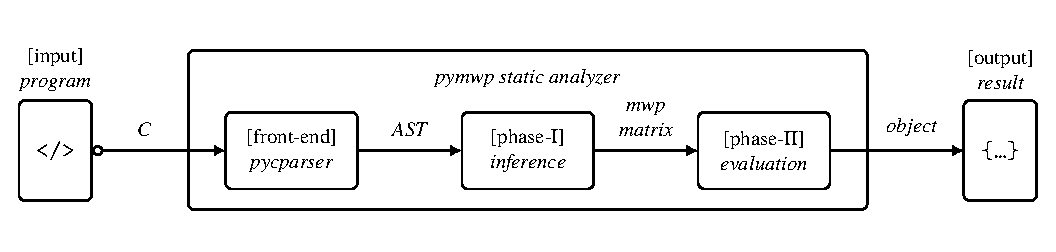
\includegraphics[width=\textwidth,keepaspectratio]{fig_pymwp}
\caption[The pymwp static analyzer workflow.]{
The pymwp\index{pymwp} static analyzer workflow.
pymwp analyzes a C\index{C}\index{programming language!C} program
and produces a result with information about the program's variable value growth.
If the program is derivable\index{derivability}, the result contains mwp-bounds\index{mwp-bound} for all variables.
Otherwise, the result identifies the variables with problematic data flows that cause derivation failure.
}\label{fig:pymwp}
\end{figure}

\paragraph*{Postconditions via mwp-bounds.}\index{mwp-bound}
The most recent development applies the flow calculus\index{mwp-calculus} to specification inference, namely postconditions~\cite{rusch2025}.
This ia new use-case, shifting the focus form static analysis toward formal verification.
Technically it introduces three flow calculus\index{mwp-calculus} enhancements:
projecting the mwp analysis on individual variables, improving the derivation failure handling strategy, an evaluation strategy to obtain optimal mwp-bounds\index{mwp-bound} through a query procedure.
For example, it permits inferring mwp-bounds\index{mwp-bound} of some variables in presence of whole-program derivation failure.
Due to focus on verifying numerical loops, the programming language is restricted to a language of loops.
The language adjustment is now a prerequisite to obtain the technical enhancements.
The loop analysis variant is implemented in pymwp\index{pymwp} as a special mode called mwp\(_\ell\).

\begin{table}[p]
\resizebox{\textwidth}{!}{%
\begin{NiceTabular}{l|l@{}}
\toprule
\textbf{0. The original flow calculus}
&
\textbf{1. The enhanced \textsc{mwp}\(^\infty\) calculus} \\
\midrule
\begin{tabular}{@{}ll}
    Motivation & complexity theory \\ \\[.5em]
    \multicolumn{2}{@{}l}{\textsc{Analysis input}} \\
    Language & \(\mathcal{L}\) (baseline)\tabularnote{
        The baseline language \(\mathcal{L}\) is similar to the
        imperative language IMP, appearing in~\textcite{nielson2010,cpierce20221}.} \\[.5em]
    \multicolumn{2}{@{}l}{\textsc{Analysis procedure}} \\
    Calculus variant & \textsc{mwp} \\
    Matrix type & simple flows \\
    Matrix count & 0--\(3^k\) \\
    Failure recovery & complete restart \\
    Failure feedback & none \\[.5em]
    \multicolumn{2}{@{}l}{\textsc{Analysis output}} \\
    Discovery procedure & immediate \\
    Bound output & arbitrary \\
    Bounds granularity  & whole-program \\
    Implementation & none \\
\end{tabular}
&
\begin{tabular}{@{}ll}
    Motivation & complexity theory \\
    & to static analysis \\[.5em]
    \multicolumn{2}{@{}l}{\textsc{Analysis input}}\\
    Language & \(\mathcal{L} + f +\) recursion \\[.5em]
    \multicolumn{2}{@{}l}{\textsc{Analysis procedure}} \\
    Calculus variant & \textsc{mwp}\(^\infty\)  \\
    Matrix type &  complex \\
    Matrix count & 1 \\
    Failure recovery & \(\infty\) \\
    Feedback report & none  \\[.5em]
    \multicolumn{2}{@{}l}{\textsc{Analysis output}} \\
    Discovery procedure & brute force  \\
    Bound output  & exists (y/n)\tabularnote{
        The analysis determines if a bound exists, but does not provide mwp-bounds by default.} \\
    Bounds granularity  & whole-program \\
    Implementation & pymwp 0.1.6 \\
\end{tabular} \\
\midrule
\textbf{2. The pymwp static analyzer}
&
\textbf{3. Postconditions via mwp-bounds}\index{mwp-bound} \\
\midrule
\begin{tabular}{@{}ll}
    Motivation &  static analysis \\[.5em]
    \multicolumn{2}{@{}l}{\textsc{Analysis input}} \\
    Language & \(\mathcal{L} \mapsto \) C99 \\[.5em]
    \multicolumn{2}{@{}l}{\textsc{Analysis procedure}} \\
    Calculus variant & \textsc{mwp}\(^\infty\)  \\
    Matrix type &  complex \\
    Matrix count & 1 \\
    Failure recovery & \(\infty\) \\
    Feedback report & failing variables  \\[.5em]
    \multicolumn{2}{@{}l}{\textsc{Analysis output}} \\
    Discovery procedure & evaluation  \\
    Bound output  & arbitrary \\
    Bounds granularity  & whole-program \\
    Implementation & pymwp 0.4.2 \\
\end{tabular}
&
\begin{tabular}{@{}ll}
    Motivation & verification \\[.5em]
    \multicolumn{2}{@{}l}{\textsc{Analysis input}} \\
    Language & loops \(\subset \mathcal{L}\) \\[.5em]
    \multicolumn{2}{@{}l}{\textsc{Analysis procedure}} \\
    Calculus variant & \textsc{mwp}\(^\infty\)  \\
    Matrix type &  complex \\
    Matrix count & 1 \\
    Failure recovery & \(\infty\) \\
    Feedback report & failing variables  \\[.5em]
    \multicolumn{2}{@{}l}{\textsc{Analysis output}} \\
    Discovery procedure & evaluation  \\
    Bound output  & optimal \\
    Bounds granularity  & variables \\
    Implementation & mwp\(_\ell\) 0.5.4 \\
\end{tabular}
\\ \bottomrule
\end{NiceTabular}}
\caption[Technical developments of the flow calculus of mwp-bounds.]
{Comparison of technical developments and features in works extending the flow calculus of mwp-bounds.}
\label{tab:evo}
\index{imperative programs}
\index{complexity theory}
\index{mwp-calculus}
\index{pymwp}
\index{C}\index{programming language!C}
\end{table}

\paragraph*{Open problems for future developments.}
Throughout the technical progression, the class of programs covered by the analysis has remained similar;
with small adjustments.
The semantic property of interest, variable value growth \wrt inputs, is never lost nor altered.
% -- the goal is consistently bounding variable value growth \wrt inputs.
Therefore, the flow calculus\index{mwp-calculus} input/output behavior has remained the same.
All notable changes concern the mechanics of the analysis and how to improve the process by which the analysis arrives to its conclusion.
In the original mwp-calculus\index{mwp-calculus}, determining program derivability\index{derivability} is an NP-complete\ccxi{np} problem.
It is unknown if the efficiency has changed following the technical advancements.

Among the remaining open problems are:
\begin{enumerate*}
\item extending the imperative language\index{imperative programs} to cover a larger class of programs,
\item formally verifying the flow calculus\index{mwp-calculus} for obtain a rigorous soundness guarantee (\cf~\autoref{coqpl}),
\item exploring the extended analysis applications, and
\item enhancing the precision of the flow calculus\index{mwp-calculus}.
\end{enumerate*}
Matrix construction is currently the most costly analysis phase.
It is possible to design data flows that make program analysis inefficient due to the resulting matrix size.
More effort is needed to scale the analysis to such inputs.

\subsubsection{Sound and Compositional Static Program Analysis}\label{mwp-analysis}

The flow calculus\index{mwp-calculus} provides a static technique for analyzing programs written in an imperative language\index{imperative programs}.
Through its inference rules\index{inference rule}, the analysis assigns coefficients\index{flow coefficient} to program commands to determine if the program is derivable\index{derivability}.
This section gives an overview of the program analysis mechanics that suffices to understand the derivation examples that follow.
We present the original flow calculus\index{mwp-calculus}, because it generates mwp-matrices of simple coefficients which are easier to present and discuss on paper.
In contrast, the \textsc{mwp}\(^\infty\) calculus\index{mwp-calculus} generates complex mwp-matrices that requires two program analysis phases, for mwp-matrix\index{mwp-matrix} construction and evaluation.
For the best exposition of how to construct complex mwp-matrices see~\aref{sec:fscd}.
The evaluation procedure that extracts mwp-bounds\index{mwp-bound} from complex mwp-matrices is best described in~\autoref{sec:postcond}.

\paragraph*{Imperative programming language.}
The imperative language\index{imperative programs} specifies the inputs of the analysis.
The language and semantics are defined in several dissertation manuscripts (\cf~\autoref{sec:postcond} and~\aref{sec:fscd}, also~\cite[p. 4]{jones2009}) thus not repeated here.
A \emph{program} is a sequence of commands.
A program manipulates sequentially a fixed number of natural number variables,
with conditional branching and iteration permitted.
Control expressions in \pr|if| statements and \pr|while| loops do not matter;
all branches are analyzed and \pr|while| loops are over-approximated to iterate infinitely.
Conventionally, a program in the flow calculus\index{mwp-calculus} corresponds to a procedure.
Although simple, the imperative language\index{imperative programs} captures a core fragment of mainstream programming languages,
like C\index{C}\index{programming language!C}
and  Java\index{Java}\index{programming language!Java},
and makes all languages that share the same core analyzable.

\paragraph*{The mwp-matrix algebra.}\index{mwp-matrix}
We use the definitions from the original flow calculus\index{mwp-calculus}~\cite{jones2009}.
The mwp-matrix algebra provides a mathematical framework for tracking variable value growth.

\begin{description}
\item[Elements.]
The mwp-matrix\index{mwp-matrix} elements are coefficients\index{flow coefficient} (or \emph{scalars}) in \(\mathcal{V} = \{ 0, m, w, p \} \).
The elements in \(\mathcal{V}\) are ordered \( 0 < m < w < p \) and letters \(\alpha, \beta, \gamma, \ldots\) denote elements in \(\mathcal{V}\).
The least upper bound of \(\alpha, \beta \in \mathcal{V}\) is denoted by \(\alpha + \beta\).
The operation evaluates to \(\alpha + \beta = \alpha\) if \(\alpha \geq \beta\), otherwise \(\alpha + \beta = \beta\).
The product of \(\alpha, \beta \in \mathcal{V}\) is denoted by \(\alpha \times \beta\) and
defined by  \(\alpha \times \beta = \alpha + \beta\) if \(\alpha, \beta \in \{m, w, p\}\),
otherwise \(\alpha \times \beta = 0\).

\begin{figure}
\begin{center}
$\begin{pNiceMatrix}[first-row,first-col]
& \prm{X}_0 & \hdots & \prm{X}_n \\
\prm{X}_0  & \ddots &      &  \iddots \\
\vdots  &  &  \alpha  & \\
\prm{X}_n & \iddots &      & \ddots
\end{pNiceMatrix}$
\end{center}
\caption{Variables labeling an mwp-matrix\index{mwp-matrix}.}
\label{fig:labels}
\end{figure}

\item[Matrices.]
For a program with \(n\) variables, an mwp-matrix\index{mwp-matrix}
\item (denoted \(M, A, B, C, \ldots\)) is a \(n \times n\) matrix over \(\mathcal{V}\).
We use \(M_{ij}\) to denote the matrix element at \emph{row} \({i}\) and \emph{column} \({j}\).
A \emph{zero matrix}\index{zero matrix} is denoted by \({0}\) and defined by \(M=0\) iff \(M_{ij} = 0\) for all indices \(i, j\).
An \emph{identity matrix}\index{identity matrix} is denoted by \({1}\) and defined by \(M = 1\) iff \(M_{ij} = m\) for \(i = j\) and \(M_{ij} = 0\) for \(i \neq j\).
The matrices are labelled by the program variables, as shown in~\autoref{fig:labels}, though the labels are typically omitted for compactness in derivations.
If no labels are provided, assume ascending alphabetical ordering of variables by default.

\item[Matrix operations.]\index{mwp-matrix}
The least upper bound \( A \oplus B \) of the matrices \(A\) and \(B\) is defined component wise,
\ie \(C = A \oplus B\) iff \(C_{ij} =A_{ij} + B_{ij}\) for \(i, j \in \{ 1,\ldots,n \}\).
The matrix product \( A \otimes B \) of the matrices \(A\) and \(B\) is defined by \(M = A \otimes B \) iff \(M_{ij} = \Sigma_{k=1\ldots n} A_{ik} \times B_{kj}\), \ie standard matrix multiplication.
The closure (fixed point) of the matrix \(M\) is denoted by \(M^*\) and
defined as an infinite sum \[M^* = 1 \oplus M \otimes M^2 \oplus M^3 \oplus \ldots \]
\end{description}

\paragraph*{The inference rules of the mwp-calculus.}
\index{inference rule}
\index{mwp-calculus}

\begin{figure}
\begin{subfigure}{\textwidth}
\begin{center}
\begin{tabular}{l}
\begin{prooftree}[small]
\infer0[E1]{ \vdashJK \text{\pr|Xi|} : \{_{\text{\,\pr|i|}}^{m}\}}
\end{prooftree}
\hspace{2em}
\begin{prooftree}[small]
\infer0[E2]{ \vdashJK \text{\pr|e|} : \{_{\text{\,\pr|i|}}^{w} \mid \text{\pr|Xi|} \in \var(\text{\pr|e|}) \}}
\end{prooftree}
\end{tabular}
\end{center}
\end{subfigure}
\\[1.2em]
\begin{subfigure}{\textwidth}
\begin{center}
\begin{tabular}{l}
\begin{prooftree}[small]
\hypo{\vdashJK \text{\pr{Xi}} : V_1}
\hypo{\vdashJK \text{\pr{Xj}} : V_2}
\infer[left label={\(\star\in\{+, -\}\)}]2[E3]{\vdashJK \text{\pr|Xi $\star$ Xj|} : pV_1 \oplus V_2}
\end{prooftree}
\hspace{1em}
\begin{prooftree}[small]
\hypo{\vdashJK \text{\pr{Xi}} : V_1}
\hypo{\vdashJK \text{\pr{Xj}} : V_2}
\infer[left label={\(\star\in\{+, -\}\)}]2[E4]{\vdashJK \text{\pr|Xi $\star$ Xj|} : V_1 \oplus pV_2}
\end{prooftree}
\end{tabular}
\end{center}
\caption{Rules for assigning vectors to expressions}
\label{fig:rules-expressions}
\end{subfigure}
\\[3em]
\begin{subfigure}{\textwidth}
\begin{centering}
\begin{prooftree}[small]
\infer0[S]{ \vdashJK \text{\pr|skip|} : \mathbf{1} }
\end{prooftree}
\hspace{3em}
\begin{prooftree}[small]
\hypo{ \vdashJK \text{\pr{e}} : V}
\infer1[A]{\vdashJK \text{\pr|Xj = e|} : \mathbf{1} \xleftarrow{\text{\pr|j|}} V}
\end{prooftree}
\hspace{3em}
\begin{prooftree}[small]
\hypo{ \vdashJK \text{\pr{C1}} : M_1}
\hypo{ \vdashJK \text{\pr{C2}} : M_2}
\infer2[C]{\vdashJK \text{\pr{C1;C2}} : M_1 \otimes M_2}
\end{prooftree}
\\[1.2em]
\begin{prooftree}[small]
\hypo{ \vdashJK \text{\pr{C1}} : M_1}
\hypo{ \vdashJK \text{\pr{C2}} : M_2}
\infer2[I]{\vdashJK \text{\pr|if b then C1 $\text{\hspace{.3em}}$ else C2|} : M_1 \oplus M_2}
\end{prooftree}
\\[1.2em]
\begin{prooftree}[small]
\hypo{\vdashJK \text{\pr|C|} : M}
\infer[left label={\(\forall i, M_{ii}^* = m\)}]1[L]{\vdashJK \text{\pr|loop Xl \{C\}|} : M^* \oplus \{_{\text{\pr|l|}}^{p}\rightarrow j \mid \exists i, M_{ij}^* = p\}}
\end{prooftree}
\\[1.2em]
\begin{prooftree}[small]
\hypo{\vdashJK \text{\pr|C|} : M}
\infer[left label={\(\forall i, M_{ii}^* = m\) and \(\forall i, j, M^*_{ij} \neq p\)}]1[W]{\vdashJK \text{\pr|while b do  \{C\}|} : M^*}
\end{prooftree}
\caption{Rules for assigning matrices to commands}
\label{fig:rules-commands}
\end{centering}
\end{subfigure}
\caption{The nondeterministic inference rules of the original mwp-calculus.}
\label{fig:jkrules}\index{inference rule}\index{nondeterminism}
\end{figure}

The inference rules\index{inference rule} of the mwp-calculus\index{mwp-calculus} \cf~\autoref{fig:jkrules} specify how different program operations impact variable value growth during computation.
Effectively, they provide the mechanics for connecting the mwp-matrix\index{mwp-matrix} algebra with imperative programs\index{imperative programs}.

\begin{description}
\item[Expressions.]
An \emph{expression} \pr|e| is assigned a vector \(V\) of coefficients\index{flow coefficient} \(\prm{e} : V\).
The rules for analysing expressions, E1--E4, are defined in~\autoref{fig:rules-expressions}.
The notation \(\{_{i}^{\alpha}\}\) means a vector with \(\alpha\) in its \(i^\text{th}\) row and $0$ everywhere else, and \(\var(\prm{e})\) means variables occurring in \pr|e|.
The product \(\alpha V\), where \(\alpha\) is a coefficient\index{flow coefficient} and \(V\) is a vector, is defined by
standard scalar multiplication of the vector elements.
Observe that there are 3 ways to analyze a binary operation.
This is the source of nondeterminism\index{nondeterminism} in the flow calculus\index{mwp-calculus}.
For \(k\) binary operation in the input program, there are \(3^k\) different derivation paths to analyze.
\item[Commands.]
A \emph{command} \pr|C| is assigned a (\(n \times n\)) matrix\index{mwp-matrix} \(M\) of coefficients\index{flow coefficient} \(\prm{C} : M\).
The rules for analysing commands are defined in~\autoref{fig:rules-commands}.
The notation \(M \xleftarrow{j} V\) means replacing in matrix $M$ the \(j^\text{th}\) column vector by $V$.
The notation \(_{\text{\pr|l|}}^{p}\rightarrow j\) means adding coefficient \(p\) in column \(j\) at row \pr|l|,
where \pr|l| is the column index of the loop guard variable\index{guard variable} \pr|Xl|.
\end{description}
The assignment rule A has the effect that the \emph{source} variables in the assignment expression impact the value growth of the assignment \emph{target}.
By the composition rule C, the impact of a command sequence is the product of the mwp-matrices\index{mwp-matrix} of the commands.
Since matrix multiplication is not commutative, the command order is relevant in mwp-calculus\index{mwp-calculus}.
The rule for \pr|if| statements accounts for computations in both branches, irrespective or order.
Only the iterative commands, \pr|loop| and \pr|while| have side conditions.
This means if a derivation fails, the source of failure is an iteration command.
Similarly, proving that variable value growth is polynomially bounded is trivial in absence of iteration.
Between the two iteration commands, \pr|while| is less permissive as it does not permit any \(p\)-flows in the mwp-matrix\index{mwp-matrix}.
The \pr|skip| command is simply an identity matrix\index{identity matrix} and has no effect.
However, it is necessary to formally handle \eg an omitted \pr|else| branch.
The \pr|skip| also permits handling commands that have no impact on variable value growth,
but that occur in realistic programming languages, \eg assertions.

\paragraph*{The analysis procedure.}
Recall, a program is a sequence of commands.
Program analysis using the flow calculus\index{mwp-calculus} requires inspecting the sequence of commands,
applying the inference rules\index{inference rule}, and composing the mwp-matrices of the commands.
Each command is either derivable\index{derivability} or raises a derivation failure.

In practice, the analysis is performed over the program's abstract syntax tree\index{abstract syntax tree} (AST).
Since a tree is a hierarchical structure, the analysis proceeds in depth-first order, like evaluation of a sequential program.
The derivation examples in~\autoref{mwp-derivations} demonstrate the concept.
For simplicity, in describing the analysis procedure we assume a flattened parse-tree of commands.

Let \(P = (\prm{C}_0,\prm{C}_1,\ldots,\prm{C}_m) \) be a program in an imperative language\index{imperative programs} where \(m \geq 1\).
A generalized program analysis proceeds by~\autoref{alg:prog}, with the analysis of individual commands is described in~\autoref{alg:comms}\footnote{
    Detailed implementations of these algorithms are available in the pymwp\index{pymwp} source code as
    \href{https://github.com/statycc/pymwp/blob/40c9ceb644c734f15f82e63edc515716c4f35841/pymwp/analysis.py\#L118}
    {\pr|Analysis.cmds|} and
    \href{https://github.com/statycc/pymwp/blob/40c9ceb644c734f15f82e63edc515716c4f35841/pymwp/analysis.py\#L185}{\pr|Analysis.compute\_relation|}.}.
Conceptually, the program analysis is straightforward: compose the mwp-matrices of commands in the order they appear in the AST\@.
However, in practice care is needed to account for the exponential number of derivation paths
and handling potential derivation failure.
Failure handling varies between the different versions of the flow analysis (\cf~\autoref{tab:evo});
therefore, the specifics are omitted here.
The \textsc{mwp}\(^\infty\) variant of the flow calculus\index{mwp-calculus} internalizes the failure and always returns an mwp-matrix\index{mwp-matrix}.

\begin{algorithm}
\caption{Program analysis with flow calculus of mwp-bounds.}\label{alg:prog}
\textbf{Input}: sequence of commands \pr|P| \\
\textbf{Output}: mwp-matrix\index{mwp-matrix} \(M\) or failure
\begin{algorithmic}[1]
\State Take the first command \(\prm{C}_0\) in \(P\)
\State Analyze \(\prm{C}_0\) by \autoref{alg:comms}
\State (Maybe signal failure)
\For{Commands \(n = 1 \ldots m\)}
\State Analyze \(\prm{C}_n\) by \autoref{alg:comms}
\State (Maybe signal failure)
\State Compose \(M = M \circ M_n \) by rule C
\EndFor
\State \Return Matrix \(M\) \Comment{\(\vdash P : M\)}
\end{algorithmic}
\end{algorithm}

\begin{algorithm}
\caption{Command analysis with flow calculus of mwp-bounds.}\label{alg:comms}
\textbf{Input}: command \pr|C| \\
\textbf{Output}: mwp-matrix\index{mwp-matrix} \(M\) or failure
\begin{algorithmic}[1]
\State Analyze expressions in \pr|C| by rules E1-E4
\State Analyze \pr|C| by rules A-W possibly recursively
\State (Maybe signal failure)
\State \Return \(M\) \Comment{\(\vdash\prm{C} : M\)}
\end{algorithmic}
\end{algorithm}

\subsubsection{Illustrative Derivations I: The Range of Analysis Outcomes}\label{mwp-derivations}

\begin{example}[Polynomially bounded program is derivable]\label{ex:bounds1T}
Recall the program from~\autoref{ex:bounds1},

\lstinputlisting[
language=IMP,
caption={A derivable program.}
]{derivable.c}

The conclusion about derivability\index{derivability} can be reached by $3^2 = 9$ distinct derivations,
one of which is shown below.

\begin{center}\begin{prooftree}
\infer0[E1]{\vdashJK \text{\pr|X2|} : \mat{0\\m\\0}}
\infer0[E1]{\vdashJK \text{\pr|X3|} : \mat{0\\0\\m}}
\infer2[E4]{\vdashJK \text{\pr|X2+X3|} : \mat{0\\m\\p}}
\infer1[A]{ \vdashJK \text{\pr|X1=X2+X3|} : \mat{0&0&0 \\ m&m&0 \\p&0&m}}
\infer0[E1]{\vdashJK \text{\pr|X1|} : \mat{m\\0\\0}}
\infer0[E1]{\vdashJK \text{\pr|X1|} : \mat{m\\0\\0}}
\infer2[E4]{\vdashJK \text{\pr|X1+X1|} : \mat{p\\0\\0}}
\infer1[A]{ \vdashJK \text{\pr|X1=X1+X1|} : \mat{p&0&0 \\ 0&m&0 \\0&0&m}}
\infer2[C]{\vdashJK \text{\pr|X1=X2+X3; X1=X1+X1|} :  \mat{0&0&0 \\ p&m&0 \\p&0&m}}
\end{prooftree}\end{center}

The mwp-bounds\index{mwp-bound} are obtained column-wise from the concluding mwp-matrix\index{mwp-matrix}, cf.~\autoref{interpreting-bounds}.
For \pr|X1|, the vector \(\mat{0\\p\\p}\)
corresponds to \(x_1' \leq \max(0) + \prm{X2}\times\prm{X3}\) and simplifies to \(x_1' \leq\prm{X2}\times\prm{X3}\).
The mwp-bound\index{mwp-bound} is not as tight as possible (expression \pr|X2+X3| would be an improvement),
but discovering a better one requires exploring the derivation paths exhaustively.
Variables \pr|X2| and \pr|X3| obtain the same mwp-bounds\index{mwp-bound} in every derivation.
For \pr|X2|, the vector \(\mat{0\\m\\0}\) gives an mwp-bound\index{mwp-bound} \(x_2' \leq\prm{X2}\),
and for \pr|X3|, the vector \(\mat{0\\0\\m}\) gives \(x_3' \leq\prm{X3}\).
The program bound is a conjunction of the variables' mwp-bounds\index{mwp-bound}, \ie
\(x_1'\leq\prm{X2}\times\prm{X3} \land x_2' \leq\prm{X2} \land x_3' \leq\prm{X3}\).
\end{example}

\begin{example}[Failing program admits no derivation]\label{ex:bounds2F}
Consider the program fragment from~\autoref{ex:bounds2},

\lstinputlisting[
language=IMP,
caption={A loop that always fails the derivation.}
]{failing.c}

The command \pr|X1=X1+X1| admits three derivations.

\begin{center}
\begin{prooftree}
\infer0[E1]{ \vdashJK \text{\pr|X1|} : \mat{m\\0}}
\infer1[E3]{ \vdashJK \text{\pr|X1+X1|} : \mat{p\\0}}
\infer1[A]{ \vdashJK \text{\pr|X1=X1+X1|} : \mat{p&0\\0&m}}
\end{prooftree}
\hfill
\begin{prooftree}
\infer0[E1]{ \vdashJK \text{\pr|X1|} : \mat{m\\0}}
\infer1[E4]{ \vdashJK \text{\pr|X1+X1|} : \mat{p\\0}}
\infer1[A]{ \vdashJK \text{\pr|X1=X1+X1|} : \mat{p&0\\0&m}}
\end{prooftree}
\hfill
\begin{prooftree}
\infer0[E2]{ \vdashJK \text{\pr|X1+X1|} : \mat{w\\0}}
\infer1[A]{ \vdashJK \text{\pr|X1=X1+X1|} : \mat{w&0\\0&m}}
\end{prooftree}
\end{center}

The next step in the derivation requires accounting for the enclosing loop by applying the rule L.
The application involves computing the closure (fixed point) \(M^{*}\) of the mwp-matrix\index{mwp-matrix} assigned to
the body command \pr|X1=X1+X1|.
In this instance, the fixed point computation does not change the mwp-matrix\index{mwp-matrix} coefficients\index{flow coefficient}.
The L side condition is \(\forall i, M_{ii}^* = m\).
That is, it requires \(m\)-coefficients on the diagonal of \(M^{*}\).
None of the derivations satisfy the side condition, therefore the program is not derivable\index{derivability}.
Although the analysis focused only on a program fragment,
the complete program fails because it contains a command that is not derivable\index{derivability}.
\end{example}

\begin{example}[Derivability in presence of partial derivation failure]\label{ex:partial}
\index{derivability}
Consider the following program, that is a slightly modified version of~\autoref{ex:bounds2F},

%! suppress = FileNotFound
\lstinputlisting[language=IMP,caption={A loop that fails along some derivation paths.},label={lst:partial-fail}]{partial.c}

The body of the \pr|loop| command admits three different derivations,
obtained by applying the tule A to one of the three derivation of the expression
\pr|X1+X2|, that we name \(\pi_0\), \(\pi_1\) and \(\pi_2\):

\begin{center}
\scalebox{0.85}{
\begin{prooftree}[small]
    \infer0[E1]{ \vdashJK \text{\pr|X1|} : \mat{m\\0\\0}}
    \infer0[E1]{ \vdashJK \text{\pr|X2|} : \mat{0\\m\\0}}
    \infer2[E3]{ \vdashJK \text{\pr|X1+X2|} : \mat{p\\m\\0}}
\end{prooftree}}
\hfill
\scalebox{0.85}{
\begin{prooftree}[small]
    \infer0[E1]{ \vdashJK \text{\pr|X1|} : \mat{m\\0\\0}}
    \infer0[E1]{ \vdashJK \text{\pr|X2|} : \mat{0\\m\\0}}
    \infer2[E4]{ \vdashJK \text{\pr|X1+X2|} : \mat{m\\p\\0}}
\end{prooftree}}
\hfill
\scalebox{0.85}{
\begin{prooftree}[small]
    \infer0[E2]{ \vdashJK \text{\pr|X1+X2|} : \mat{w\\w\\0}}
\end{prooftree}}
\end{center}

From \(\pi_0\), the derivation of  \pr|loop X3 {X2=X1+X2}| can be
completed using A and L, but since L requires having only \(m\) coefficients
on the diagonal, \(\pi_1\) cannot be used to complete the derivation,
because of the \(p\) coefficient in a box below:

\begin{center}
\begin{prooftree}
\hypo{}
\ellipsis{\(\pi_0\)}{ \vdashJK \text{\pr|X1+X2|} : \mat{p\\m\\0}}
\infer1[A]{ \vdashJK \text{\pr|X2=X1+X2|} : \mat{m&p&0 \\ 0&m&0 \\0&0&m}}
\infer1[L]{ \vdashJK \text{\pr|loop X3 \{X2=X1+X2\}|} :  \mat{m&p&0 \\ 0&m&0 \\0&p&m}}
\end{prooftree}
\hspace{2em}
\begin{prooftree}
\hypo{}
\ellipsis{\(\pi_1\)}{ \vdashJK \text{\pr|X1+X2|} : \mat{m\\p\\0}}
\infer1[A]{ \vdashJK \text{\pr|X2=X1+X2|}: \mat{m&m&0 \\ 0& \boxed{p} &0 \\0&0&m}}
\end{prooftree}
\end{center}

Similarly, using A after \(\pi_2\) gives a \(w\) coefficient on the
diagonal and makes it impossible to use L, hence only one derivation for this program exists.
A single successful derivation is sufficient to make the input program derivable\index{derivability}.
\end{example}

\subsubsection{Illustrative Derivations II: Programs From the Tool User Guide}

The pymwp\index{pymwp} tool user guide, in ~\autoref{app:toolguide}, discusses five cases of program analysis of programs written in C\index{C}\index{programming language!C}.
The tool user guide gives the analyzer input and output and describes the rationale for the obtained result.
This section complements the tool user guide by showing the derivations behind those results.
To retail fidelity with the C\index{C}\index{programming language!C} language examples,
we show inputs in C\index{C}\index{programming language!C},
but implicitly convert them to the core imperative language\index{imperative programs} of the flow calculus\index{mwp-calculus}.
The examples omit function declarations since those are irrelevant for the analysis.

\begin{example}[Binary assignment]\label{ex:binassign}
The input program

\begin{minipage}{\textwidth}
\lstinputlisting[
language=C,
caption={A program with a single assignment.}
]{assign_expression.c}
\end{minipage}

contains a single command.
The program has three derivations and all of them succeed.
One derivation instance is shown below.

\begin{center}\begin{prooftree}
\infer0[E1]{\vdashJK \text{\pr|Y1|} : \mat{m\\0}}
\infer0[E1]{\vdashJK \text{\pr|Y1|} : \mat{m\\0}}
\infer2[E3]{\vdashJK \text{\pr|Y1+Y1|} : \mat{p\\0}}
\infer1[A]{ \vdashJK \text{\pr|Y2=Y1+Y1|} : \mat{0&p \\m&0}}
\end{prooftree}\end{center}
The program bound is a \(y_1'\leq\prm{Y1} \land y_2' \leq\prm{Y1}\).
\end{example}

\begin{example}[Exponential Program]\label{ex:expprog}
The input program is

\begin{minipage}{\textwidth}
\lstinputlisting[
language=C,
caption={A program with exponential variable value growth.}
]{exponent2.c}
\end{minipage}

\paragraph*{Step 1.} Analyze the command \pr|r=r*b|.
It admits three derivations (\(\pi_0\), \(\pi_1\) and \(\pi_2\)).

\begin{center}
\scalebox{0.85}{
\begin{prooftree}[small]
\infer0[E1]{ \vdashJK\text{\pr|r|} : \mat{0\\0\\0\\m}}
\infer0[E1]{ \vdashJK\text{\pr|b|} : \mat{m\\0\\0\\0}}
\infer2[E3]{ \vdashJK\text{\pr|r*b|} : \mat{p\\0\\0\\m}}
\infer1[A]{ \vdashJK\text{\pr|r=r*b|} : \mat{m&0&0&p\\0&m&0&0\\0&0&m&0\\0&0&0&m}}
\end{prooftree}}
\hfill
\scalebox{0.85}{
\begin{prooftree}[small]
\infer0[E1]{ \vdashJK \text{\pr|r|} : \mat{0\\0\\0\\m}}
\infer0[E1]{ \vdashJK \text{\pr|b|} : \mat{m\\0\\0\\0}}
\infer2[E4]{ \vdashJK \text{\pr|r*b|} : \mat{m\\0\\0\\p}}
\infer1[A]{ \vdashJK\text{\pr|r=r*b|} : \mat{m&0&0&m\\0&m&0&0\\0&0&m&0\\0&0&0&p}}
\end{prooftree}}
\hfill
\scalebox{0.85}{
\begin{prooftree}[small]
\infer0[E2]{ \vdashJK \text{\pr|r*b|} : \mat{w\\0\\0\\w}}
\infer1[A]{ \vdashJK\text{\pr|r=r*b|} : \mat{m&0&0&w\\0&m&0&0\\0&0&m&0\\0&0&0&w}}
\end{prooftree}}
\end{center}

\paragraph*{Step 2.} Analyze command \pr|i=i+1|.
Similarly, it admits three derivations (\(\pi_3\), \(\pi_4\) and \(\pi_5\)).

\begin{center}
\scalebox{0.85}{
\begin{prooftree}[small]
\infer0[E1]{ \vdashJK \text{\pr|i|} : \mat{0\\0\\m\\0}}
\infer0[E1]{ \vdashJK \text{\pr|1|} : \mat{0\\0\\0\\0}}
\infer2[E3]{ \vdashJK \text{\pr|i+1|} : \mat{0\\0\\p\\0}}
\infer1[A]{ \vdashJK \text{\pr|i=i+1|} : \mat{m&0&0&0\\0&m&0&0\\0&0&p&0\\0&0&0&m}}
\end{prooftree}}
\hfill
\scalebox{0.85}{
\begin{prooftree}[small]
\infer0[E1]{ \vdashJK \text{\pr|i|} : \mat{0\\0\\m\\0}}
\infer0[E1]{ \vdashJK \text{\pr|1|} : \mat{0\\0\\0\\0}}
\infer2[E4]{ \vdashJK \text{\pr|i+1|} : \mat{0\\0\\m\\0}}
\infer1[A]{ \vdashJK \text{\pr|i=i+1|} : \mat{m&0&0&0\\0&m&0&0\\0&0&m&0\\0&0&0&m}}
\end{prooftree}}
\hfill
\scalebox{0.85}{
\begin{prooftree}[small]
\infer0[E2]{ \vdashJK \text{\pr|i+1|} : \mat{0\\0\\w\\0}}
\infer1[A]{ \vdashJK \text{\pr|i=i+1|} : \mat{m&0&0&0\\0&m&0&0\\0&0&w&0\\0&0&0&m}}
\end{prooftree}}
\end{center}

\paragraph*{Step 3.} Compose the body commands, \pr|r=r*b; i=i+1|.
There are 9 different combinations, by the derivation choices made in the previous steps.

\begin{center}
\begin{prooftree}
\hypo{}\ellipsis{\(\pi_0\times\pi_3\)}{ }
\infer1[C]{ \vdashJK \text{\pr|B|} : \mat{m&0&0&p\\0&m&0&0\\0&0&p&0\\0&0&0&m}}
\end{prooftree}
\hfill
\begin{prooftree}
\hypo{}\ellipsis{\(\pi_0\times\pi_4\)}{ }
\infer1[C]{ \vdashJK \text{\pr|B|} : \mat{m&0&0&p\\0&m&0&0\\0&0&m&0\\0&0&0&m}}
\end{prooftree}
\hfill
\begin{prooftree}
\hypo{}\ellipsis{\(\pi_0\times\pi_5\)}{ }
\infer1[C]{ \vdashJK \text{\pr|B|} : \mat{m&0&0&p\\0&m&0&0\\0&0&w&0\\0&0&0&m}}
\end{prooftree}
\\[1em]
\begin{prooftree}
\hypo{}\ellipsis{\(\pi_1\times\pi_3\)}{ }
\infer1[C]{ \vdashJK \text{\pr|B|} : \mat{m&0&0&m\\0&m&0&0\\0&0&p&0\\0&0&0&p}}
\end{prooftree}
\hfill
\begin{prooftree}
\hypo{}\ellipsis{\(\pi_1\times\pi_4\)}{ }
\infer1[C]{ \vdashJK \text{\pr|B|} : \mat{m&0&0&m\\0&m&0&0\\0&0&m&0\\0&0&0&p}}
\end{prooftree}
\hfill
\begin{prooftree}
\hypo{}\ellipsis{\(\pi_1\times\pi_5\)}{ }
\infer1[C]{ \vdashJK \text{\pr|B|} : \mat{m&0&0&m\\0&m&0&0\\0&0&w&0\\0&0&0&p}}
\end{prooftree}
\\[1em]
\begin{prooftree}
\hypo{}\ellipsis{\(\pi_2\times\pi_3\)}{ }
\infer1[C]{ \vdashJK \text{\pr|B|} : \mat{m&0&0&w\\0&m&0&0\\0&0&p&0\\0&0&0&w}}
\end{prooftree}
\hfill
\begin{prooftree}
\hypo{}\ellipsis{\(\pi_2\times\pi_4\)}{ }
\infer1[C]{ \vdashJK \text{\pr|B|} : \mat{m&0&0&w\\0&m&0&0\\0&0&m&0\\0&0&0&w}}
\end{prooftree}
\hfill
\begin{prooftree}
\hypo{}\ellipsis{\(\pi_2\times\pi_5\)}{ }
\infer1[C]{ \vdashJK \text{\pr|B|} : \mat{m&0&0&w\\0&m&0&0\\0&0&w&0\\0&0&0&w}}
\end{prooftree}
\end{center}

\paragraph*{Step 4.}
Apply rule W to account for the enclosing \pr|while| loop.
It requires first computing mwp-matrix\index{mwp-matrix}  closure \(M^{*}\) for the body command.
The side conditions is \(\forall i, M_{ii}^* = m\) and \(\forall i, j, M^*_{ij} \neq p\).
That is, the rule can be applied when only $m$-coefficients appear on the diagonal
and no $p$-coefficients occur anywhere in the mwp-matrix\index{mwp-matrix} .
In every derivation, the mwp-matrix\index{mwp-matrix}  violates the side condition by the boxed coefficients\index{flow coefficient}.

\begin{center}
\begin{prooftree}
\hypo{}\ellipsis{\(\pi_0\times\pi_3\)}{M^{*} = \mat{m&0&0&\boxed{p}\\0&m&0&0\\0&0&\boxed{p}&0\\0&0&0&m}}
\end{prooftree}
\hfill
\begin{prooftree}
\hypo{}\ellipsis{\(\pi_0\times\pi_4\)}{M^{*} = \mat{m&0&0&\boxed{p}\\0&m&0&0\\0&0&m&0\\0&0&0&m}}
\end{prooftree}
\hfill
\begin{prooftree}
\hypo{}\ellipsis{\(\pi_0\times\pi_5\)}{M^{*} = \mat{m&0&0&\boxed{p}\\0&m&0&0\\0&0&\boxed{w}&0\\0&0&0&m}}
\end{prooftree}
\\[1em]
\begin{prooftree}
\hypo{}\ellipsis{\(\pi_1\times\pi_3\)}{M^{*} = \mat{m&0&0&m\\0&m&0&0\\0&0&\boxed{p}&0\\0&0&0&\boxed{p}}}
\end{prooftree}
\hfill
\begin{prooftree}
\hypo{}\ellipsis{\(\pi_1\times\pi_4\)}{M^{*} = \mat{m&0&0&m\\0&m&0&0\\0&0&m&0\\0&0&0&\boxed{p}}}
\end{prooftree}
\hfill
\begin{prooftree}
\hypo{}\ellipsis{\(\pi_1\times\pi_5\)}{M^{*} = \mat{m&0&0&m\\0&m&0&0\\0&0&\boxed{w}&0\\0&0&0&\boxed{p}}}
\end{prooftree}
\\[1em]
\begin{prooftree}
\hypo{}\ellipsis{\(\pi_2\times\pi_3\)}{M^{*} = \mat{m&0&0&w\\0&m&0&0\\0&0&\boxed{p}&0\\0&0&0&\boxed{w}}}
\end{prooftree}
\hfill
\begin{prooftree}
\hypo{}\ellipsis{\(\pi_2\times\pi_4\)}{M^{*} = \mat{m&0&0&w\\0&m&0&0\\0&0&m&0\\0&0&0&\boxed{w}}}
\end{prooftree}
\hfill
\begin{prooftree}
\hypo{}\ellipsis{\(\pi_2\times\pi_5\)}{M^{*} = \mat{m&0&0&w\\0&m&0&0\\0&0&\boxed{w}&0\\0&0&0&\boxed{w}}}
\end{prooftree}
\end{center}

\paragraph*{Step 5.} We conclude the input program is not derivable\index{derivability}.
\end{example}

\begin{example}[While analysis]\label{ex:while1}
The input program, that we will refer to as \(P\), is

\begin{minipage}{\textwidth}
%! suppress = FileNotFound
\lstinputlisting[
language=C,
caption={While loop analysis.}
]{notinfinite3.c}
\end{minipage}

The tool user guide reveals that the program is derivable\index{derivability}.
Compared to derivation failure that requires exploring all derivation choices,
a derivable\index{derivability} program simply requires showing one successful derivation.
For presentation reasons, we show the two branches of the derivation tree individually.

\paragraph*{Step 1.} The derivation of the \pr|if| command (\(\pi_0\)){ }is straightforward.
Observe that the control expression of the \pr|if| statement has no impact on the constructed mwp-matrix\index{mwp-matrix}.

\begin{center}
\begin{prooftree}
\infer0[E1]{\vdashJK \text{\pr|X1|} : \mat{0\\m\\0\\0}}
\infer0[E1]{\vdashJK \text{\pr|X2|} : \mat{0\\0\\m\\0}}
\infer2[E4]{\vdashJK \text{\pr|X2+X1|} : \mat{0\\m\\p\\0}}
\infer1[A]{ \vdashJK \text{\pr|X1=X2+X1|} : \mat{m&0&0&0\\0&m&0&0\\0&p&m&0\\0&0&0&m}}
\infer0[E1]{\vdashJK \text{\pr|X3|} : \mat{0\\0\\0\\m}}
\infer0[E1]{\vdashJK \text{\pr|X2|} : \mat{0\\0\\m\\0}}
\infer2[E4]{\vdashJK \text{\pr|X3+X2|} : \mat{0\\0\\m\\p}}
\infer1[A]{ \vdashJK \text{\pr|X2=X3+X2|} : \mat{m&0&0&0\\0&m&0&0\\0&0&m&0\\0&0&p&m}}
\infer2[I]{ \vdashJK \text{\pr|if(X1==1) \{ X1=X2+X1; X2=X3+X2 \}|} : \mat{m&0&0&0\\0&m&0&0\\0&p&m&0\\0&0&p&m}}
\end{prooftree}
\end{center}

\paragraph*{Step 2.} The derivation of the \pr|while| loop (\(\pi_1\)){ }is now permitted,
because the rule W side condition is not violated by any coefficient\index{flow coefficient}.

\begin{center}
\begin{prooftree}
\infer0[E1]{\vdashJK \text{\pr|X1|} : \mat{0\\w\\0\\0}}
\infer0[E1]{\vdashJK \text{\pr|X2|} : \mat{0\\0\\w\\0}}
\infer2[E4]{\vdashJK \text{\pr|X1+X2|} : \mat{0\\w\\w\\0}}
\infer1[A]{ \vdashJK \text{\pr|X0=X1+X2|} : \mat{0&0&0&0\\w&m&0&0\\w&0&m&0\\0&0&0&m}}
\infer1[W]{ \vdashJK \text{\pr|while(X0<10) X0=X1+X2 |} : \mat{m&0&0&0\\w&m&0&0\\w&0&m&0\\0&0&0&m}}
\end{prooftree}
\end{center}

\paragraph*{Step 3.} Composing the mwp-matrices of the two commands
gives an mwp-matrix\index{mwp-matrix} for the complete input program \(P\).
We conclude the syntactic data-flow relation\index{data flow relation} \(\vdash P : M \) holds.

\begin{center}
\begin{prooftree}
\hypo{}
\ellipsis{\(\pi_0\times\pi_1\)}{ }
\infer1[C]{\vdashJK P : \mat{m&0&0&0\\w&m&0&0\\p&p&m&0\\p&0&p&m}}
\end{prooftree}
\end{center}
If the program terminates\index{termination} for the input values of the variables (it does not terminate for all inputs),
the variable value growth is polynomially bounded.
The mwp-bounds\index{mwp-bound} of the variables are
\(x_0' \leq \max(\prm{X0},\prm{X1})+\prm{X2}\times\prm{X3}\) and
\(x_1' \leq \max(\prm{X1})+\prm{X2} \) and
\(x_2' \leq \max(\prm{X2})+\prm{X3} \) and
\(x_3' \leq \max(\prm{X3})\).
This program bound matches the result of the tool user guide.
\end{example}

\begin{example}[Infinite program]\label{ex:infprog}
The input program is

\begin{minipage}{\textwidth}
%! suppress = FileNotFound
\lstinputlisting[
language=C,
caption={An \enquote{infinite} program.}
]{infinite3.c}
\end{minipage}

This program is similar to~\autoref{ex:while1}, with only a small change to the \pr|while| loop.
From the previous example, the \pr|if| statement is derivable\index{derivability} as before by \(\pi_0\).
Letting \(\prm{C}_2\) represent the \pr|while| command, the mwp-matrix\index{mwp-matrix} closures \(M^{*}\) of \(\prm{C}_2\) are shown below.

\begin{center}
\begin{prooftree}
\hypo{}\ellipsis{E3}{M^{*} = \mat{m&0&0&0\\0&\boxed{p}&0&0\\0&m&m&0\\0&0&0&m}}
\end{prooftree}
\hfill
\begin{prooftree}
\hypo{}\ellipsis{E4}{M^{*} = \mat{m&0&0&0\\0&m&0&0\\0&\boxed{p}&m&0\\0&0&0&m}}
\end{prooftree}
\hfill
\begin{prooftree}
\hypo{}\ellipsis{E2}{M^{*} = \mat{m&0&0&0\\0&\boxed{w}&0&0\\0&w&m&0\\0&0&0&m}}
\end{prooftree}
\end{center}
Every \(M^{*}\) violates the side condition of rule W.
The problematic coefficient\index{flow coefficient} is boxed for emphasis.
The program is not derivable\index{derivability}.
\end{example}

\begin{example}[Challenge example]\label{ex:challange}
The input program has four top-level commands, identified by the circled annotations.

\begin{minipage}{\textwidth}
%! suppress = FileNotFound
\lstinputlisting[
language=C,escapeinside=||,
caption={A challenge program that may, or may not, be derivable.},
label={lst:maybe-derivable}]{dense_loop.c}
\end{minipage}

We will refer to these commands as \(\prm{C}_0\)--\(\prm{C}_3\) and
their derivations as \(\pi_0\)--\(\pi_3\), respectively.
The program analysis proceeds in corresponding steps.
To ease presentation, we will analyze command composition after each individual command.

\paragraph*{Step 1.} Analyze command \(\prm{C}_0\) \ie the \pr|if-else| statement.

\begin{center}\begin{prooftree}
\infer0[E1]{\vdashJK \text{\pr|X0|} : \mat{m\\0\\0}}
\infer0[E1]{\vdashJK \text{\pr|X1|} : \mat{0\\m\\0}}
\infer2[E4]{\vdashJK \text{\pr|X0+X1|} : \mat{m\\p\\0}}
\infer1[A]{ \vdashJK \text{\pr|X2=X0+X1|} : \mat{m&0&m\\0&m&p\\0&0&0}}
\infer0[E1]{\vdashJK \text{\pr|X2|} : \mat{0\\0\\m}}
\infer0[E1]{\vdashJK \text{\pr|X1|} : \mat{0\\m\\0}}
\infer2[E4]{\vdashJK \text{\pr|X2+X1|} : \mat{0\\p\\m}}
\infer1[A]{ \vdashJK \text{\pr|X2=X2+X1|} : \mat{m&0&0\\0&m&p\\0&0&m}}
\infer2[I]{ \vdashJK \text{\pr|if(X0) X2=X0+X1; else X2=X2+X1|} : \mat{m&0&m\\0&m&p\\0&0&m}}
\end{prooftree}\end{center}

\paragraph*{Steps 2--3.} Analyze commands \(\prm{C}_1\) and \(\prm{C}_2\), \ie \pr|X0=X2+X1| and \pr|X1=X0+X2|.

\begin{center}
\begin{prooftree}
\infer0[E1]{\vdashJK \text{\pr|X2|} : \mat{0\\0\\m}}
\infer0[E1]{\vdashJK \text{\pr|X1|} : \mat{0\\m\\0}}
\infer2[E4]{\vdashJK \text{\pr|X2+X1|} : \mat{0\\p\\m}}
\infer1[A]{\vdashJK \text{\pr|X0=X2+X1|} : \mat{0&0&0\\p&m&0\\m&0&m}}
\end{prooftree}
\hfill
\begin{prooftree}
\infer0[E2]{\vdashJK \text{\pr|X0+X2|} : \mat{w\\0\\w}}
\infer1[A]{\vdashJK \text{\pr|X1=X0+X2|} : \mat{m&w&0\\0&0&0\\0&w&m}}
\end{prooftree}
\end{center}

\paragraph*{Steps 4.} Analyze command \(\prm{C}_3\) \ie the \pr|while| loop.

\begin{center}
\begin{prooftree}
\infer0[E2]{\vdashJK \text{\pr|X1+X0|} : \mat{w\\w\\0}}
\infer1[A]{\vdashJK \text{\pr|X2=X1+X0|} : \mat{m&0&w\\0&m&w\\0&0&0}}
\infer1[W]{ \vdashJK \text{\pr|while(X2) X2=X1+X0|} : \mat{m&0&w\\0&m&w\\0&0&m}}
\end{prooftree}
\end{center}

\paragraph*{Steps 5.} Compose the mwp-matrices of derivations \(\pi_0 \ldots \pi_3\).

\noindent\resizebox{\textwidth}{!}{\begin{prooftree}
\hypo{}\ellipsis{\(\pi_0\)}{\vdashJK \prm{C}_0 : \mat{m&0&m\\0&m&p\\0&0&m}}
\hypo{}\ellipsis{\(\pi_1\)}{\vdashJK \prm{C}_1 : \mat{0&0&0\\p&m&0\\m&0&m}}
\infer2[C]{ \vdashJK \prm{C}_0\prm{;}\prm{C}_1 : \mat{m&0&m\\p&m&p\\m&0&m}}
\hypo{}\ellipsis{\(\pi_2\)}{\vdashJK \prm{C}_2 : \mat{m&w&0\\0&0&0\\0&w&m}}
\infer2[C]{ \vdashJK \prm{C}_0\prm{;}\prm{C}_1\prm{;}\prm{C}_2 : \mat{m&w&m\\p&p&p\\m&w&m}}
\hypo{}\ellipsis{\(\pi_3\)}{\vdashJK \prm{C}_3  : \mat{m&0&w\\0&m&w\\0&0&m}}
\infer2[C]{ \vdashJK \prm{C}_0\prm{;}\prm{C}_1\prm{;}\prm{C}_2\prm{;}\prm{C}_3 :
\mat{m&w&w\\p&p&p\\m&w&w}}
\end{prooftree}}

\vspace{1em}\noindent
The derivation gives variable mwp-bounds\index{mwp-bound}
\(x_0' \leq \max(\prm{X0},\prm{X2})+\prm{X1}\) and
\(x_1' \leq \prm{X0}+\prm{X2}+\prm{X1}\) and
\(x_2' \leq \prm{X0}+\prm{X2}+\prm{X1}\).
The program has 81 admissible derivations in total.
\end{example}